Majoritatea sistemelor de tip interfon, chiar si cele nou instalate, sunt realizate cu terminale de telefonie fixa datorita simplitudinii modului de operare. In esenta este nevoie de 4 fire pentru a avea o linie de telecomunicatie bi-directionala.

\href{https://www.epanorama.net/documents/telecom/telephone_intercom.html}{Simple schema}

\begin{figure}[h!]
  \centering
  \fbox {
    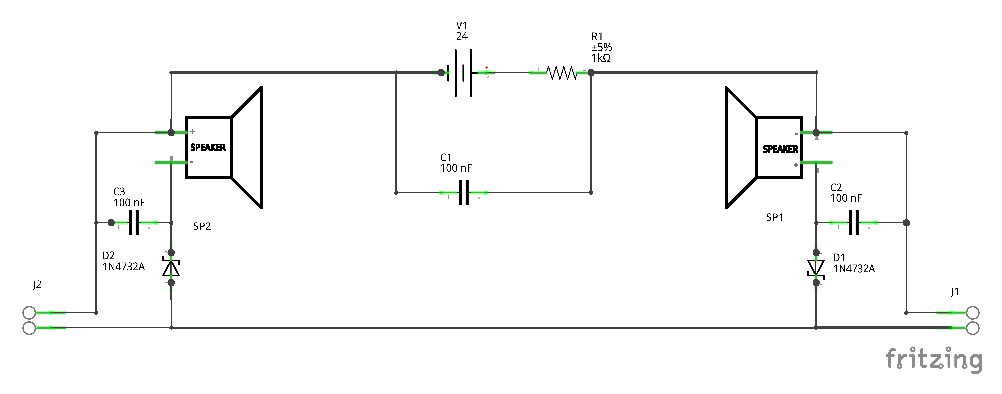
\includegraphics[width=0.8\textwidth]{01/interfon_schem.pdf}  
  }
  \caption{Schema simpla interfon cu speaker}
\end{figure}

\section {Plain Ordinary Telephone System}

Pentru a adauga mai multe terminale in retea, a fost dezvoltata tehnologia numita POTS (Plain Ordinary Telephone Service). Coordonarea acestui sistem este realizata de un decodor DTMF ce are rolul de a transforma semnalul modulat de pe linia X intr-o adresa din retea. 

\begin{figure}[h!]
  \centering
  \fbox {
    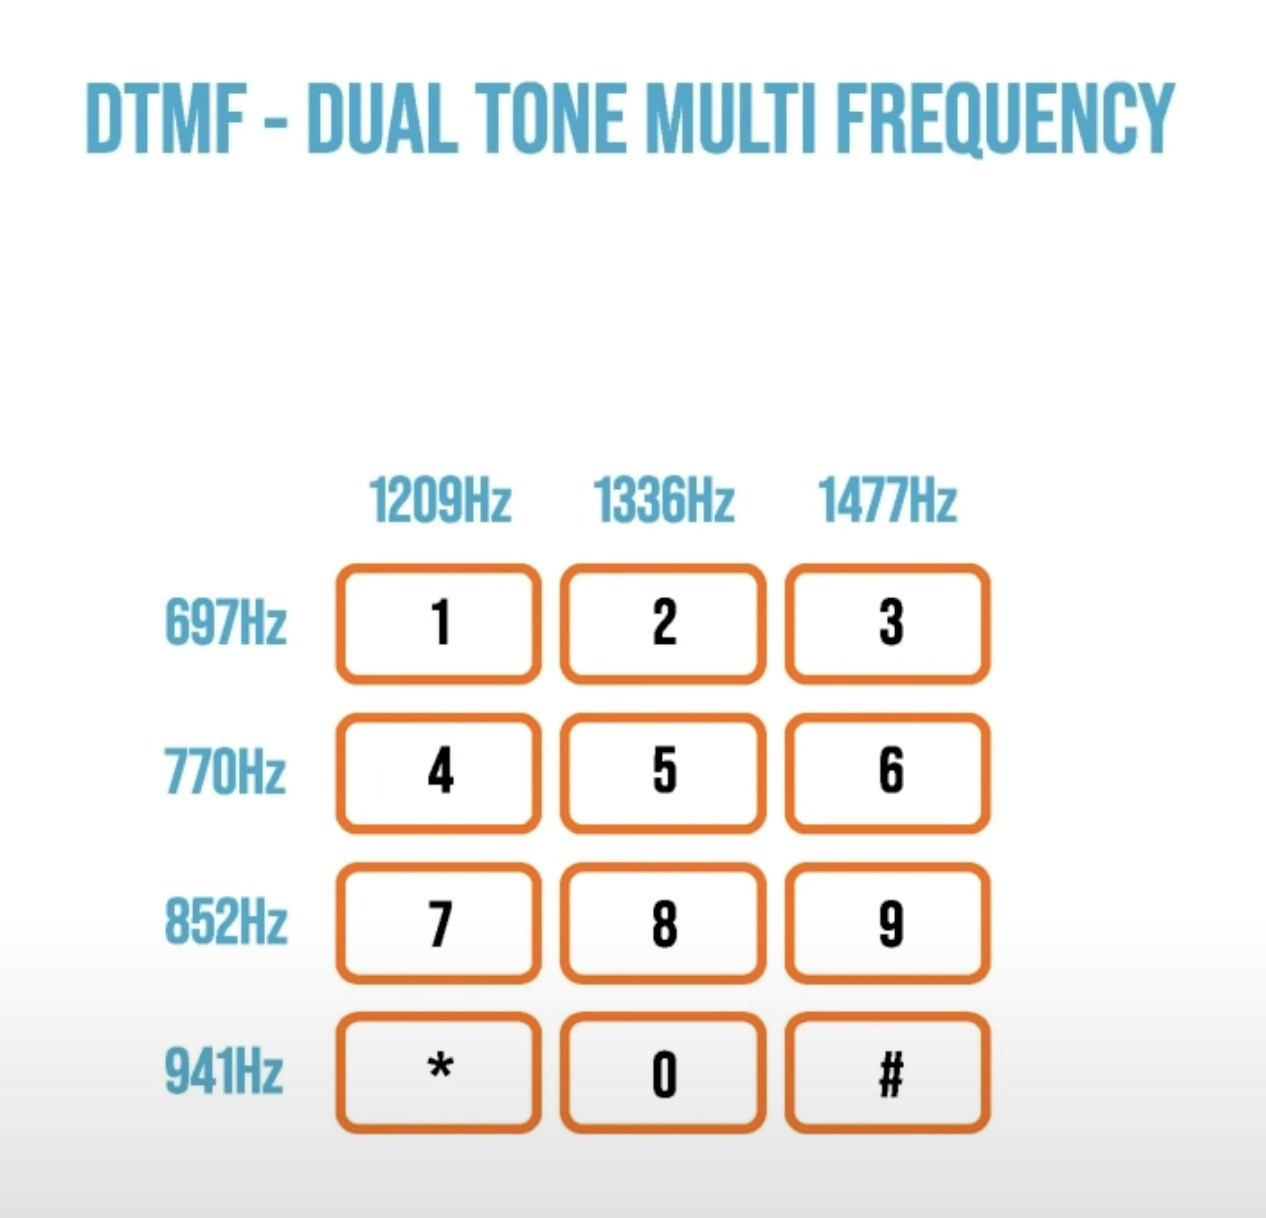
\includegraphics[width=0.8\textwidth]{01/dtmf.jpeg}  
  }
  \caption{Diagrama DTMF}
\end{figure}

In DTMF randurile sunt numite si GROUP JOS (cu frecvente intre 600 si 900 $Hz$), iar coloanele sunt numite GROUP INALT. Asadar, cand se apasa tasta 8 a unui terminal, frecventa de $852 Hz$ este aleasa din grupulul JOS si frecventa $1336 Hz$ sunt emise in acelasi timp.


Decodorul DTMF foloseste filtre Notch pentru acest procedeu.

\begin{figure}[h!]
  \centering
  \fbox {
    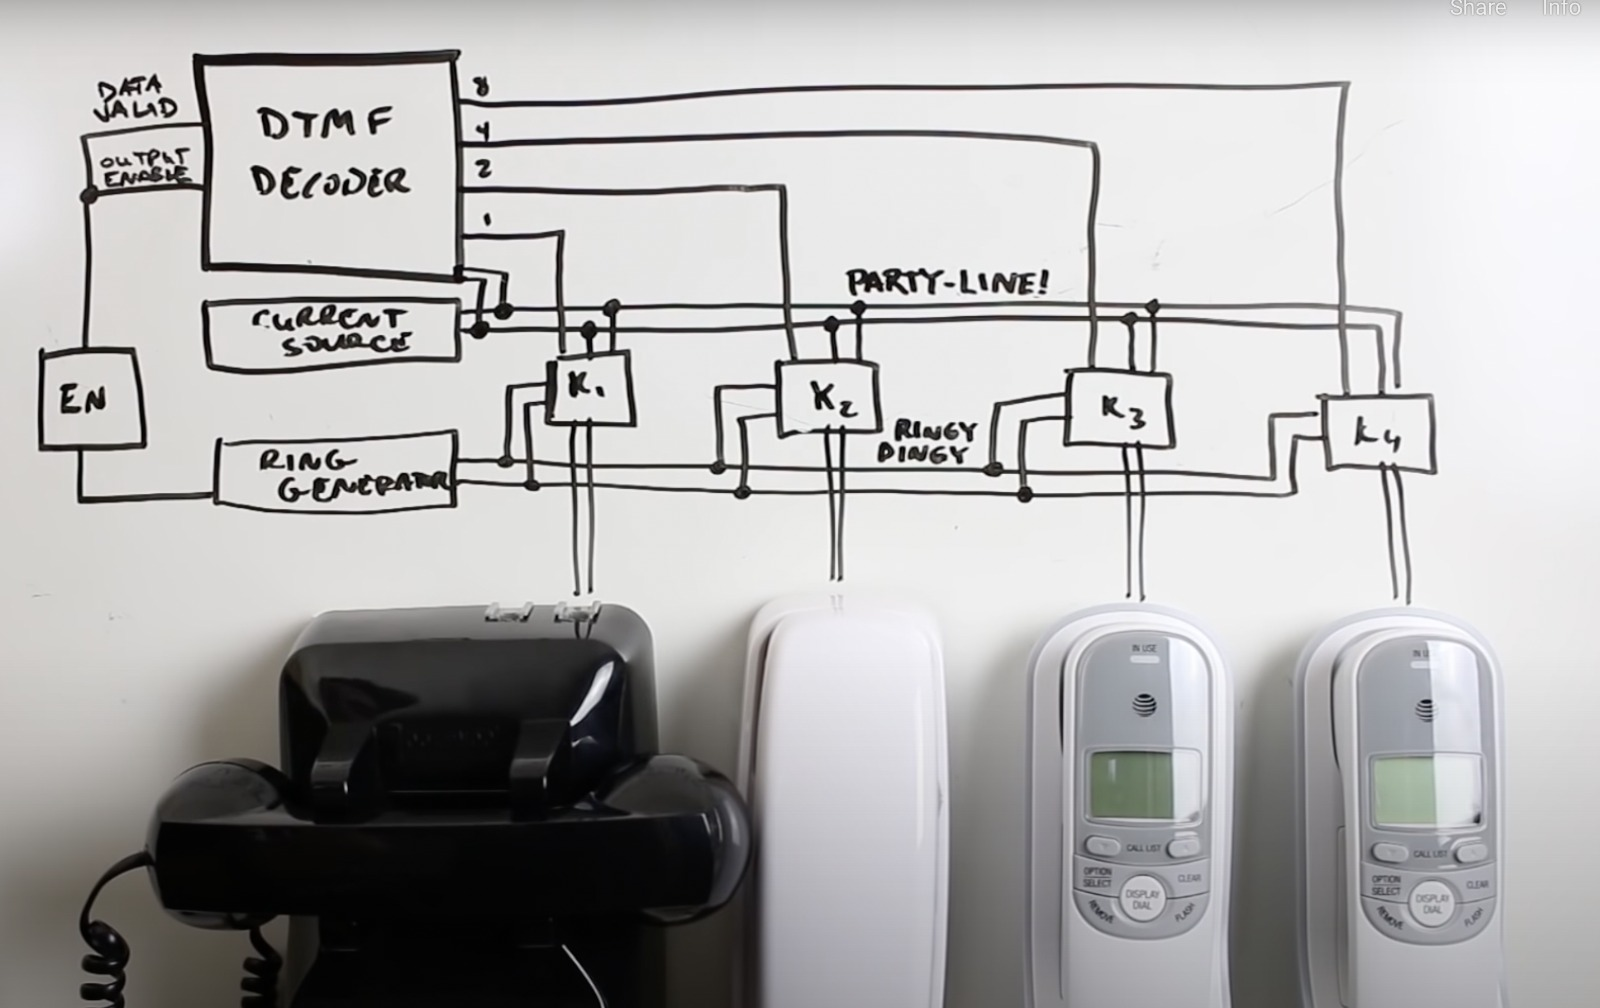
\includegraphics[width=0.8\textwidth]{01/schema_pots.jpeg}  
  }
  \caption{Schema sistem POTS}
\end{figure}

\cite{WinNT}



\href{https://www.nextiva.com/blog/what-is-pots.html}{Alt articol}

O evolutie normala de la acest sistem, ca si trecerea de la telefonul fix la cel mobil, sunt interfoanele GSM. Acestea dispun de un modul GSM cu o agenda ce are rolul de a oferi acces numerelor salvate sa interactioneze cu sistemul.


\section {Videx UK}

\href{https://www.videxuk.com/system/gsm-intercoms/}{Videx UK}


\section {Interfon GSM}

\href{https://www.a2t.ro/interfoane-videointerfoane/interfon-wireless-gsm-pentru-o-familie.html}{Link}

Interfon wireless GSM pentru o familie si controlere GSM pentru deschidere de porti sau bariere. Foarte util pentru zonele in care nu exista cablaje. Poate deschide o yala, o automatizare sau o bariera. Vorbesti cu vizitatorii direct de pe telefonul tau mobil. Functioneaza pe reteaua oricarui operator de telefonie mobila 2G.

\section {Hikvision DS-KV8413-WME1}

\href{https://www.a2t.ro/videointerfon-wireless/videointerfon-full-hd-4-familii-control-acces-aplicat-tcp-ip-hikvision-ds-kv8413-wme1-s.html}{Link}

\href{https://www.hikvision.com/content/dam/hikvision/products/S000000001/S000000083/S000000129/S000000131/OFR000170/M000048926/User_Manual/UD20207B_Baseline_Video-Intercom-8-Series-Villa-Door-Station_User-Manual_V2.2.3.PDF}{Manual}


Post de exterior, camera 2MP, WiFi Proxi, 4 butoane de apelare, reducere zgomot si ecou, audio bidirectional, BLC, DNR, WDR, IP65, IK08, PoE / 12VDC. Montaj ingropat.

Video-interfon metalic, cu 4 butoane (pentru 4 familii).